%%%%%%%%%%%%%%%%%%%%%%%%%%%%%%%%%%%%%%%%%
% Beamer Presentation
% LaTeX Template
% Version 1.0 (10/11/12)
%
% This template has been downloaded from:
% http://www.LaTeXTemplates.com
%
% License:
% CC BY-NC-SA 3.0 (http://creativecommons.org/licenses/by-nc-sa/3.0/)
%
%%%%%%%%%%%%%%%%%%%%%%%%%%%%%%%%%%%%%%%%%

%----------------------------------------------------------------------------------------
%	PACKAGES AND THEMES
%----------------------------------------------------------------------------------------

\documentclass{beamer}
\mode<presentation> {
\usetheme{Madrid}
}
\usepackage{url}
\usepackage{lmodern}
\usepackage{graphicx}
\usepackage{booktabs}

% for mathematics
\usepackage{amsmath}
\usepackage{amsthm}

% for hollowed 1 (indicator variable symbol)
\usepackage{bbm}

%----------------------------------------------------------------------------------------
%	TITLE PAGE
%----------------------------------------------------------------------------------------

\title[Hawkes Process in Finance]{Hawkes Process Presentation 1} % The short title appears at the bottom of every slide, the full title is only on the title page

\author{Dong Shaocong, \\Wang Zexin} % Your name
\institute[NUS]
{
Hawkes Process in Finance\\[3mm]
\medskip
\textit{Quantitative Finance\\
National University of Singapore\\}
}
\date{\today}

\begin{document}
%----------------------------------------------------------------------------------------
%	TITLE PAGE
%----------------------------------------------------------------------------------------
\begin{frame}
\titlepage
\end{frame}

%----------------------------------------------------------------------------------------
%	TABLE OF CONTENTS
%----------------------------------------------------------------------------------------

%------------------------------------------------
\begin{frame}
\frametitle{Today's Agenda}
\tableofcontents
\end{frame}

%------------------------------------------------
\begin{frame}
\frametitle{Introduction}
\begin{itemize}
	\item Hawkes processes are a particularly interesting class of stochastic process that have been applied in diverse areas, from earthquake modelling to financial analysis.
	\item Events that are observed in time frequently cluster naturally.
	\item ``self-exciting'': Event arrival can excite the process in the sense that the chance of a subsequent arrival is increased for some time period after the initial arrival.
	\item Simple and flexible for high frequency finance.
\end{itemize}
\end{frame}

%------------------------------------------------
\section{Preliminary} %------------------------------------------------
\begin{frame}
\frametitle{Counting Process / Point Process}
Counting process is the number of arrivals until a certain point of time.\\
Arrivals are following certain prespecified distributions.
\begin{itemize}
	\item Event times: $T_i$ time of the $i$-th event
	\item $N_t = \sum_{i \ge 1} \mathbbm{1}_{\{ t \ge T_i\}}$
	\item $N_0 = 0$
	\item jump size $= 1$ at $t = T_i \; \forall i$
\end{itemize}
\end{frame}
%------------------------------------------------

\begin{frame}
\frametitle{Poisson Process}
Arrival time are distributed as exponential random variables.
\begin{itemize}
	\item $\tau_i \sim Exp(\lambda)$
	\item pdf of $\tau$ : $f_{\tau}(t) = \lambda e^{-\lambda t}, \forall t \ge 0$
	\item expectation of $\tau$ : $\mathbb{E}(\tau) = \lambda^{-1}$
	\item $T_n = \sum_{j=1}^n \tau_j$
	\item $N_t = \sum_{i \ge 1} \mathbbm{1}_{\{ t \ge T_i\}}$
	\item Memoryless property: $\mathbb{P}(\tau > t + m \mid \tau > m) = \mathbb{P}(\tau > t)$
	\item Homogeneous: all arrival times are distributed as exponential random variables with the same $\lambda$
	\item Non-Homogeneous : intensity varies with time, more formally defined as: $\lambda(t \mid H_t) = \lim_{h \to 0} \frac{\mathbb{P}\{ N_{t + h} - N_t = 1 \mid H_t\}}{h}$
\end{itemize}
\end{frame}

\section{Univariate Hawkes Process}

\begin{frame}
\frametitle{Hawkes Process}
Formulation:\\
$\lambda(t \mid F_t) = \lambda_0(t) + \sum_{i: t > T_i} \phi(t - T_i)$
\begin{itemize}
	\item $F_t$ should be recognized as a filtration, a welter of all the information known at time $t$
	\item Self-exciting property: Arrivals of events increase the likelihood of future observations. Intensity at the current time depends on how many and how far away are the most recent arrivals in the past.
	\item Non-Homogeneous, as the intensity of the exponential random variables changes with time.
	\item Deterministic base intensity function: $\lambda_0(t)$
	\item Memory Kernel: $\phi(t - T_i)$ which links to past arrivals times
	\item Event Decay: monotonically decreasing kernel
\end{itemize}
\end{frame}

\subsection{Branching Structure}
\begin{frame}
\frametitle{Branching Structure}
\begin{itemize}
	\item We can divide the events into two categories, immigrants and the offsprings.
	\item Immigrants : the events directly caused by the base intensity
	\item Offsprings : the events `\textbf{excited}' by immigrants or another offspring
	\item Self-exciting is the property which can be observed in the financial markets as momentum, in which investors following the trend in the prices tend to cause trend in the same direction.
	\item In econometrics, this property of markets is observed as reverse casuality, as price movements drive demands, and demands drive prices as well.
\end{itemize}

\begin{center}
	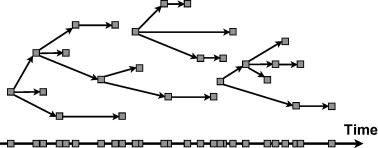
\includegraphics[scale=0.5]{image/branching_1}
\end{center}

\end{frame}

\subsection{Deterministic Intensity Functions}
\begin{frame}
\frametitle{Deterministic Intensity Functions}
Base intensity function $\lambda_0(t)>0$, describes externally triggered events (immigrants)
\begin{itemize}
	\item Independence: previous events within the process
	\item Base (or background) intensity
	\item In the multivariate/bivariate case, the intensity function can be a constant.
	\item For example, $\lambda_i,0(t) = \mu_i$ for a formulation of $\lambda_i(t) = \mu_i + \sum_{i: t > T_i} \phi(t - T_i)$
\end{itemize}
\end{frame}

\subsection{Cluster of offspring}
\begin{frame}
\frametitle{Cluster of offspring}
\begin{itemize}
	\item The offsprings of one immigrant events, which are the immediate offsprings of it, and their immediate offsprings, and their immediate offsprings, \dots, can be grouped as one cluster.
	\item Branching factor is defined as the expected number of events generated by a parent event : $\mid \Phi \mid = \int_0^{\infty} \phi(\tau) d\tau$
	\item Sub-Critical phase if $\mid \Phi \mid < 1$, meaning the number of events in one cluster is bounded.
	\item Super-Critical if $\mid \Phi \mid > 1$, meaning the number of events in one cluster is unbounded.
	\item The properties of Sub-Critical and Super-Critical mimics the stationarity property of stochastic processes.
	\item Expected number of events in one cluster $ = \frac{1}{1 - \mid \Phi \mid}$
\end{itemize}
\end{frame}

\subsection{Memory Kernels}
\begin{frame}
\frametitle{Memory Kernels}
Memory Kernels can be in any form, with two popular forms:
\begin{itemize}
	\item Exponential decay kernel: $\phi(t) = \alpha e^{-\delta t}$
	\item Power law kernel: $\phi(t) = \frac{\alpha}{(1 + \beta t)^{1 + \gamma}}$
	\item By the self-exciting property, the kernel shoud possess decay property since we expect the intensity to be higher when there are more arrivals in the near past.
	\item The multiplier $\beta$ to $\alpha$ is left out because a variable $\alpha$ is able to capture the changes by itself.
\end{itemize}
\end{frame}

\subsection{Marked Process}
\begin{frame}
	\frametitle{Marked Process}
	Each event has a corresponding mark / magnitude $m_i$ at event time $T_i$
	\begin{itemize}
		\item Event lies in domain $S \times M$
		\item power-law kernel $\phi_m(\tau) = \kappa m^{\beta}(\tau + c)^{-(1+\theta)}$
		\item Event marks $m_i$ can be i.i.d. samples from a power law distribution $P(m)=(\alpha - 1) m^{-\alpha }$
		\item Four parameters $\theta = \{\kappa,\beta,c,\theta\}$
		\begin{enumerate}
			\item $\kappa$: ``event quality'', scales the subsequent event rate
			\item $c>0$: temporal shift to keep $\phi_m(\tau)$ bounded
			\item $\theta$: power-law exponent, describing how fast an event is forgotten
		\end{enumerate}
		\item $\kappa m^{\beta}$ accounts for magnitude of influences
		\item $(\tau + c)^{-(1+\theta)}$ models the memory over time
	\end{itemize}
\end{frame}

\subsection{Simulation}

\begin{frame}
	\frametitle{Simulating events from Hawkes prosses}
	\begin{itemize}
		\item \textbf{Goal}: simulate inter-arrival times $\tau_i$, $i=1,2,\dots$, according to intensity function $\lambda_t$
		\item \textbf{Poisson Process}: $f_{\tau}(t)=\lambda e^{-\lambda t},F_{\tau}(t)=1-e^{-\lambda t} , t>0$
		\item \textit{inverse transform sampling}: $Y=F_X(X) \sim U(0,1)$ $\Rightarrow$ Sample $u\sim U(0,1)$, then compute $\tau=\frac{- \ln u}{\lambda}$
	\end{itemize}
\end{frame}

\begin{frame}
\frametitle{Thinning Algorithm - rejection sampling}
Applies to all non-homogeneous Poisson processes. 
\begin{itemize}
	\item \textit{thinning property}: Poisson process with intensity $\lambda$ can be split to two independent processes with intensities $\lambda_1$ and $\lambda_2$, where $\lambda = \lambda_1+\lambda_2$
	\item Monotonically decreasing kernel: $[T_i,T_{i+1})$, $\lambda(T_i)$ is the upper bound of event intensity.
	\item Sampling procedure:
	\begin{enumerate}
		\item $T=T_i$, sample $\tau$ (inverse transform)
		\item $\lambda^{\star}=\lambda(T)$, update $T=T+\tau$ (thinning property)
		\item $s\sim U(0,1)$, $T_i=T$ if $s<\frac{\lambda(T)}{\lambda^{\star}}$, otherwise repeat process
		\item Repeat until react to $i=N$
	\end{enumerate}
\end{itemize}
\end{frame}

\begin{frame}
\frametitle{Decomposition Algorithm}
Efficient sampling for Hawkes process with exponential kernel
\[\lambda(t)=\underbrace{a+(\lambda_0-a)e^{-\delta t}}_{\text{immigrant rate}}+\underbrace{\sum_{T_i<t}\gamma e^{-\delta(t-T_i)}}_{\text{jump by event}}, t>0 \]
\begin{itemize}
	\item Markov (process) decomposition when $\Phi$ is exponential
	\item Split to two independent parts:
	\begin{itemize}
		\item Part 1: sample $s_0=-\frac{1}{a}\ln u_0$ (inverse transform)
	\item Part 2: $s_1=-\frac{1}{\delta}\ln d$, $d=1+\frac{\delta \ln u_1}{\lambda(T^+_{i-1})-a}$ (Markov property)
	\end{itemize}
	\item Inter Arrival time = $\min\{s_0,s_1\}$ to get the first event occurring time
\end{itemize}
\end{frame}

\begin{frame}
\frametitle{Univariate Exponential Kernel Simulation}
Expected number of events with $\alpha$ varying from $0.05$ to $1$.\\
$\beta = 5, T = 10, \mu = 1$
\begin{figure}[h]
      \centering
	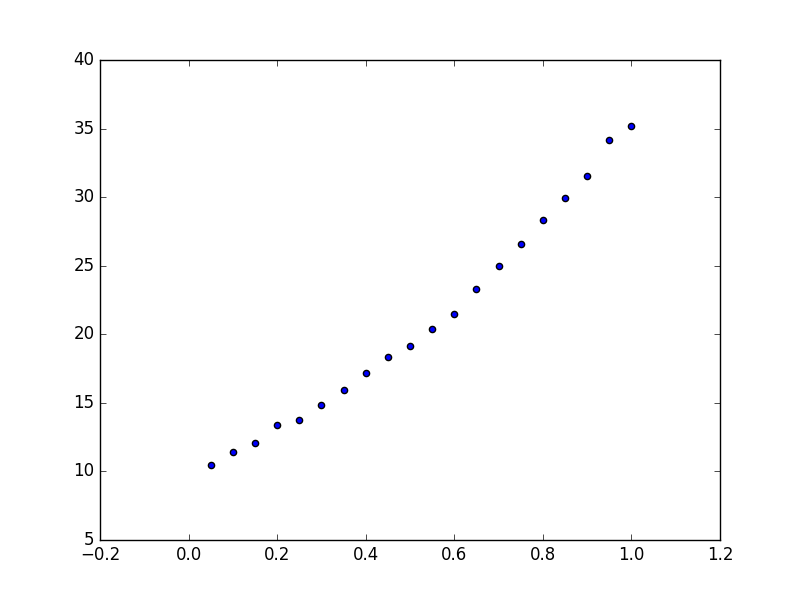
\includegraphics[scale=0.45]{image/AlphaSimulation.png}
\end{figure}
\end{frame}

\begin{frame}
\frametitle{Univariate Exponential Kernel Simulation}
Expected number of events with $\beta$ varying from $0.2$ to $4$.\\
$\alpha = 0.2, T = 10, \mu = 1$
\begin{figure}[h]
      \centering
	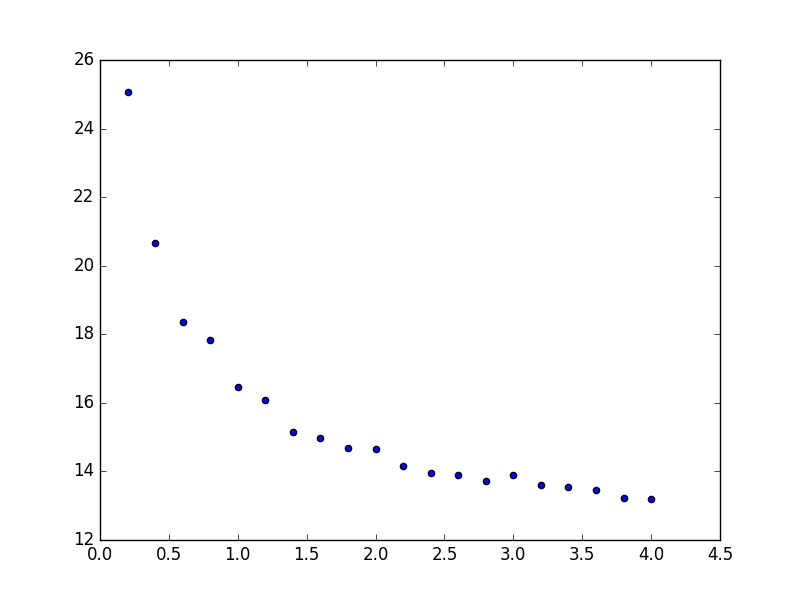
\includegraphics[scale=0.45]{image/BetaSimulation.png}
\end{figure}
\end{frame}

\begin{frame}
\frametitle{Univariate Exponential Kernel Simulation}
Expected number of events with $\mu$ varying from $0.5$ to $5$.\\
$\alpha = 0.2, \beta = 5, T = 10$
\begin{figure}[h]
      \centering
	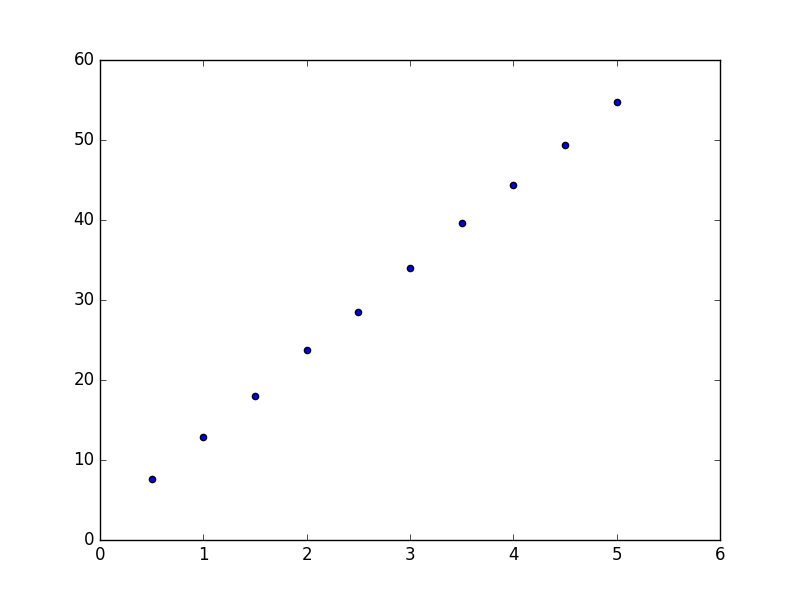
\includegraphics[scale=0.45]{image/MuSimulation.png}
\end{figure}
\end{frame}

\subsection{Parameter Estimation}
\begin{frame}
\frametitle{Likelihood functions for Exponential Kernels}
In this section we put some efforts into writing out the likelihood function of Univariate Hawkes Process, and solving for its parameters if possible and not too computationally costly.
\begin{itemize}
	\item Ideally the likehood function should be a function of the probability density functions at the event times, and the cumulative density functions between event times.
	\item $L(\Theta) = \prod_{i=1}^n f(T_{i}) \prod_{i=1}^n (1-F_{T_{i-1}}(T_i)) (1-F_{T_{n}}(T))$
	\item Cumulative density function for non-homogeneous Poisson Process can written as : $F(t) = 1 - \exp(-\int_0^t \lambda(s) ds)$, where the intensity $\lambda(s)$ is a function of time
	\item Probability density function for Hawkes Process, as we described in the previous slides, can be written as : $f(t) = \lambda(t) \exp(t\lambda(t))$, however when we let it participate in the likelihood function, $f(t) = \lambda(t)$ since the duration of event is negligible.
\end{itemize}
\end{frame}

\begin{frame}
\frametitle{Likelihood functions for Exponential Kernels}
\begin{equation*}
\begin{split}
L(\Theta) = &\prod_{i=1}^n f(T_{i}) \prod_{i=1}^n (1-F_{T_{i-1}}(T_i)) (1-F_{T_{n}}(T))\\
= &[\prod_{i=1}^n \lambda(T_{i})] [\prod_{i=1}^n \exp(-\int_{T_{i-1}}^{T_i} \lambda(s) ds)] (\exp(-\int_{T_{n}}^{T} \lambda(s) ds))\\
= &\exp(-\int_{0}^{T} \lambda(s) ds) \prod_{i=1}^n \lambda(T_{i})
\end{split}
\end{equation*}
\end{frame}

\begin{frame}
\frametitle{Likelihood functions for Exponential Kernels}
Suppose we are going to use exponential decay kernel representation and constant base intensity function:\\
$\phi(t) = \alpha e^{\delta t}$, $\lambda_0(t) = \mu \to \lambda(t \mid F_{t}) = \mu + \sum_{i: t>T_i} \alpha e^{\delta (t - T_{i})}$
\begin{equation*}
\begin{split}
L(\Theta) = &\exp(-\int_{0}^{T} \lambda(t \mid F_t) dt) \prod_{i=1}^n \lambda(T_i \mid F_{T_{i}})\\
= &\exp(-\int_{0}^{T}  \mu + \sum_{i: t>T_i} \alpha e^{\delta (t - T_i)} dt) \prod_{i=1}^n (\mu + \sum_{j=0}^i \alpha e^{\delta (T_i - T_j)})\\[5mm]
\ln L(\Theta) = & \sum_{i=1}^n \ln (\mu + \alpha \sum_{j=0}^i  e^{\delta (T_i - T_j)}) - \mu T - \alpha \int_{0}^{T}  \sum_{i: t>T_i} e^{\delta (t - T_i)} dt 
\end{split}
\end{equation*}
\end{frame}

\begin{frame}
\frametitle{Maximum Likelihood Estimates for Exponential Kernels}
Differentiate with respect to $\mu$:
\begin{equation*}
\begin{split}
\ln L(\Theta) = & \sum_{i=1}^n \ln (\mu + \alpha \sum_{j=0}^i  e^{\delta (T_i - T_j)}) - \mu T - \alpha \int_{0}^{T}  \sum_{i: t>T_i} e^{\delta (t - T_i)} dt \\
\frac{\partial}{\partial \mu} \ln L(\Theta) =& \sum_{i=1}^n \frac{1}{\mu + \alpha \sum_{j=0}^i e^{\delta (T_i - T_j)}} - T = 0\\
\to &\sum_{i=1}^n \frac{1}{\mu + \alpha \sum_{j=0}^i e^{\delta (T_i - T_j)}} = T
\end{split}
\end{equation*}
\end{frame}

\begin{frame}
\frametitle{Maximum Likelihood Estimates for Exponential Kernels}
Differentiate with respect to $\alpha$:
\begin{equation*}
\begin{split}
\ln L(\Theta) = & \sum_{i=1}^n \ln (\mu + \alpha \sum_{j=0}^i  e^{\delta (T_i - T_j)}) - \mu T - \alpha \int_{0}^{T}  \sum_{i: t>T_i} e^{\delta (t - T_i)} dt \\
\frac{\partial}{\partial \alpha} \ln L(\Theta) =& \sum_{i=1}^n \frac{e^{\delta (T_i - T_j)}}{\mu + \alpha \sum_{j=0}^i e^{\delta (T_i - T_j)}} - \int_{0}^{T}  \sum_{i: t>T_i} e^{\delta (t - T_i)} dt= 0\\
\to& \sum_{i=1}^n \frac{e^{\delta (T_i - T_j)}}{\mu + \alpha \sum_{j=0}^i e^{\delta (T_i - T_j)}} = \int_{0}^{T}  \sum_{i: t>T_i} e^{\delta (t - T_i)} dt
\end{split}
\end{equation*}
\end{frame}

\begin{frame}
\frametitle{Maximum Likelihood Estimates for Exponential Kernels}
Differentiate with respect to $\delta$:
\begin{equation*}
\begin{split}
\ln L(\Theta) = & \sum_{i=1}^n \ln (\mu + \alpha \sum_{j=0}^i  e^{\delta (T_i - T_j)}) - \mu T - \alpha \int_{0}^{T}  \sum_{i: t>T_i} e^{\delta (t - T_i)} dt \\
\frac{\partial}{\partial \delta} \ln L(\Theta) =& \sum_{i=1}^n \frac{(T_i - T_j)e^{\delta (T_i - T_j)}}{\mu + \alpha \sum_{j=0}^i e^{\delta (T_i - T_j)}} - \int_{0}^{T}  \sum_{i: t>T_i} (t - T_i)e^{\delta (t - T_i)} dt= 0\\
\to& \sum_{i=1}^n \frac{(T_i - T_j)e^{\delta (T_i - T_j)}}{\mu + \alpha \sum_{j=0}^i e^{\delta (T_i - T_j)}} = \int_{0}^{T}  \sum_{i: t>T_i} (t - T_i)e^{\delta (t - T_i)} dt
\end{split}
\end{equation*}
\end{frame}

\begin{frame}
\frametitle{Maximum Likelihood Estimates for Exponential Kernels}
\begin{equation}
\begin{split}
&\sum_{i=1}^n \frac{1}{\mu + \alpha \sum_{j=0}^i e^{\delta (T_i - T_j)}} = T
\end{split}
\end{equation}
\begin{equation}
\begin{split}
& \sum_{i=1}^n \frac{e^{\delta (T_i - T_j)}}{\mu + \alpha \sum_{j=0}^i e^{\delta (T_i - T_j)}} = \int_{0}^{T}  \sum_{i: t>T_i} e^{\delta (t - T_i)} dt
\end{split}
\end{equation}
\begin{equation}
\begin{split}
&\sum_{i=1}^n \frac{(T_i - T_j)e^{\delta (T_i - T_j)}}{\mu + \alpha \sum_{j=0}^i e^{\delta (T_i - T_j)}} = \int_{0}^{T}  \sum_{i: t>T_i} (t - T_i)e^{\delta (t - T_i)} dt
\end{split}
\end{equation}
\end{frame}

\begin{frame}
\frametitle{Likelihood functions for Power Law Kernels}
Substituting $\phi(t) = \frac{\alpha}{(1 + \beta t)^{1 + \gamma}}$ in:
\begin{equation*}
\begin{split}
L(\Theta) = &\exp(-\int_{0}^{T} \lambda(t \mid F_t) dt) \prod_{i=1}^n \lambda(T_i \mid F_{T_{i}})\\
= &\exp(-\int_{0}^{T}  \mu + \sum_{i: t>T_i} \frac{\alpha}{(1 + \beta (t - T_i))^{1 + \gamma}} dt) \\
&\prod_{i=1}^n (\mu + \sum_{j=0}^i \frac{\alpha}{(1 + \beta (T_i - T_j))^{1 + \gamma}})\\[5mm]
\ln L(\Theta) = &\sum_{i=1}^n \ln(\mu + \alpha\sum_{j=0}^i \frac{1}{(1 + \beta (T_i - T_j))^{1 + \gamma}}) - \mu T\\
- &\alpha \int_{0}^{T} \sum_{i: t>T_i} \frac{1}{(1 + \beta (t - T_i))^{1 + \gamma}} dt
\end{split}
\end{equation*}
\end{frame}

\begin{frame}
\frametitle{Maximum Likelihood Estimates for Power Law Kernels}
\begin{equation*}
\begin{split}
\ln L(\Theta) = &\sum_{i=1}^n \ln(\mu + \alpha\sum_{j=0}^i \frac{1}{(1 + \beta (T_i - T_j))^{1 + \gamma}}) - \mu T\\
- &\alpha \int_{0}^{T} \sum_{i: t>T_i} \frac{1}{(1 + \beta (t - T_i))^{1 + \gamma}} dt\\[7mm]
\frac{\partial}{\partial \mu} \ln L(\Theta) = &\sum_{i=1}^n \frac{1}{\mu + \alpha\sum_{j=0}^i \frac{1}{(1 + \beta (T_i - T_j))^{1 + \gamma}}} - T = 0\\
\end{split}
\end{equation*}
\end{frame}

\begin{frame}
\frametitle{Maximum Likelihood Estimates for Power Law Kernels}
\begin{equation*}
\begin{split}
\ln L(\Theta) = &\sum_{i=1}^n \ln(\mu + \alpha\sum_{j=0}^i \frac{1}{(1 + \beta (T_i - T_j))^{1 + \gamma}}) - \mu T\\
- &\alpha \int_{0}^{T} \sum_{i: t>T_i} \frac{1}{(1 + \beta (t - T_i))^{1 + \gamma}} dt\\[7mm]
\frac{\partial}{\partial \alpha} \ln L(\Theta) = &\sum_{i=1}^n \frac{\sum_{j=0}^i \frac{1}{(1 + \beta (T_i - T_j))^{1 + \gamma}}}{\mu + \alpha\sum_{j=0}^i \frac{1}{(1 + \beta (T_i - T_j))^{1 + \gamma}}}\\
- &\int_{0}^{T} \sum_{i: t>T_i} \frac{1}{(1 + \beta (t - T_i))^{1 + \gamma}} dt = 0\\
\end{split}
\end{equation*}
\end{frame}

\begin{frame}
\frametitle{Maximum Likelihood Estimates for Power Law Kernels}
\begin{equation*}
\begin{split}
\ln L(\Theta) = &\sum_{i=1}^n \ln(\mu + \alpha\sum_{j=0}^i \frac{1}{(1 + \beta (T_i - T_j))^{1 + \gamma}}) - \mu T\\
- &\alpha \int_{0}^{T} \sum_{i: t>T_i} \frac{1}{(1 + \beta (t - T_i))^{1 + \gamma}} dt\\[7mm]
\frac{\partial}{\partial \beta} \ln L(\Theta) = &\sum_{i=1}^n \frac{\alpha\sum_{j=0}^i \frac{T_i - T_j}{(1 + \beta (T_i - T_j))^{2 + \gamma}}}{\mu + \alpha\sum_{j=0}^i \frac{1}{(1 + \beta (T_i - T_j))^{1 + \gamma}}}\\
- &\int_{0}^{T} \sum_{i: t>T_i} \frac{t - T_i}{(1 + \beta (t - T_i))^{2 + \gamma}} dt = 0\\
\end{split}
\end{equation*}
\end{frame}

\begin{frame}
\frametitle{Univariate Model for market activity}
As tested on the 10 years Euro-Bond future front contract by Bacry, when $\gamma$ is closed to $0$, the empirical kernel is well described by the power-law kernel.
\begin{equation*}
\begin{split}
\sum_{i=1}^n \frac{1}{\mu + \alpha\sum_{j=0}^i \frac{1}{1 + \beta (T_i - T_j)}} &= T\\
\sum_{i=1}^n \frac{\sum_{j=0}^i \frac{1}{(1 + \beta (T_i - T_j))}}{\mu + \alpha\sum_{j=0}^i \frac{1}{1 + \beta (T_i - T_j)}} = &\int_{0}^{T} \sum_{i: t>T_i} \frac{1}{1 + \beta (t - T_i)} dt\\
\sum_{i=1}^n \frac{\alpha\sum_{j=0}^i \frac{T_i - T_j}{(1 + \beta (T_i - T_j))^2}}{\mu + \alpha\sum_{j=0}^i \frac{1}{1 + \beta (T_i - T_j)}} = &\int_{0}^{T} \sum_{i: t>T_i} \frac{t - T_i}{(1 + \beta (t - T_i))^2} dt\\
\end{split}
\end{equation*}
\end{frame}

\section{Bivariate Hawkes Process}

\begin{frame}
\frametitle{Bivariate / Multivariate Hawkes Process}
Formulation in our original paper:\\
$\lambda_t^i = \mu^i + \sum_{j=1}^D \int dN_{t'}^j \phi^{i,j} (t - t')$\\
\begin{itemize}
	\item $D$ : the number of variables following Hawkes Process
	\item $\phi^{i,j}$ : the effect of variable $j$'s arrival on variable $i$'s intensity
	\item $\mu^i$ : the constant base intensity function of variable $i$
	\item $\lambda_t^i$ : the intensity of variable $i$ at time $t$
	\item $T_{j,k}$ : the $k$th event time of variable $j$
\end{itemize}
Formulation after reconcilation with notation in univariate case:\\
$\lambda_t^i = \mu^i + \sum_{j=1}^2 \sum_{k: t > T_{j,k}} \phi^{i,j}(t - T_{j,k})$\\	
$\lambda_1(t \mid F_t) = \lambda_{1,0}(t) + \sum_{i: t > T_{1,i}} \phi^{1,1}(t - T_{1,i}) + \sum_{i: t > T_{2,i}} \phi^{1,2}(t - T_{2,i})$\\
$\lambda_2(t \mid F_t) = \lambda_{2,0}(t) + \sum_{i: t > T_{1,i}} \phi^{2,1}(t - T_{1,i}) + \sum_{i: t > T_{2,i}} \phi^{2,2}(t - T_{2,i})$
\end{frame}

\begin{frame}
\frametitle{Bivariate / Multivariate Hawkes Process}
\begin{itemize}
	\item Base intensity function $\lambda_{i,0}(t)>0$ describes externally triggered events (immigrants) of variable $i$
	\item The memory kernels will appear in matrix of functions, in which the functions are positive and causal
	\item $\phi^{i,j}(t) = 0 \; \forall t < 0$
	\item $\phi^{i,j}(t) >= 0 \; \forall t$
\end{itemize}
\end{frame}

\subsection{Branching Structure and Clustering Representation}
\begin{frame}
\frametitle{Branching Structure and Clustering Representation}
\begin{itemize}
	\item The different variables share the clusters, as each variable have the ability to excite other variables and own events which parent the offsprings events in other variables
\end{itemize}
\begin{figure}[h]
      \centering
	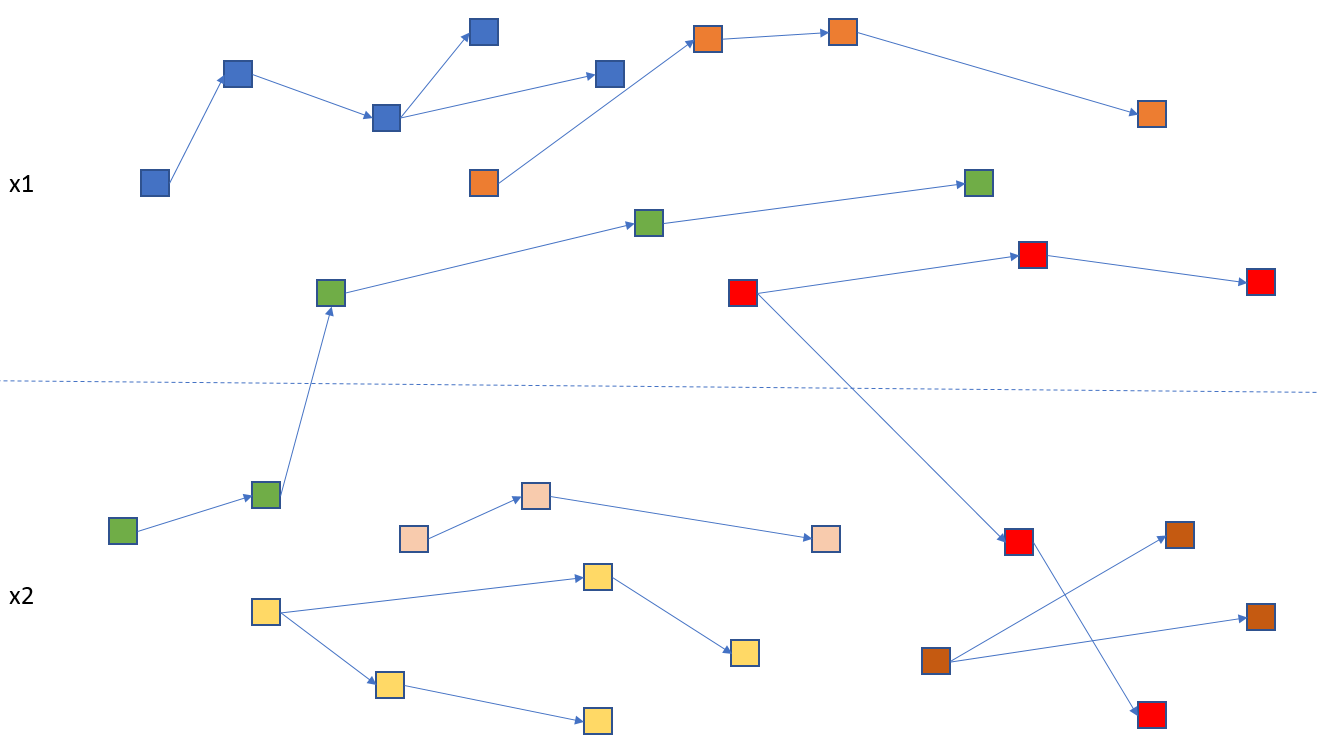
\includegraphics[scale=0.3]{image/Bivariate_Branching_Structure.png}
\end{figure}
\end{frame}

\subsection{Memory Kernels}
\begin{frame}
\frametitle{Bivariate Exponential Kernels}
\[
\Phi(t) = 
\left( \begin{array}{ccc}
\phi^s(t) & \phi^c(t) \\
\phi^c(t) & \phi^s(t) \end{array} \right).
\]
\begin{itemize}
	\item $\phi^s(t) = \alpha^s \beta^s \exp(-\beta^s t), \forall t > 0$
	\item $\phi^c(t) = \alpha^c \beta^c \exp(-\beta^c t), \forall t > 0$
	\item This is one special case, in which two variables share the same function / parameter which determine the effect of them exciting themselves or exciting the other variable.
	\item $\phi^{1,2}(t) = \phi^{2,1}(t) = \phi^s(t)$ : \textbf{s}elf-effect
	\item $\phi^{1,1}(t) = \phi^{2,2}(t) = \phi^c(t)$ : \textbf{c}ross-effect
\end{itemize}
\end{frame}

\subsection{Price Model}
\begin{frame}
\frametitle{Bivariate Price Model}
\begin{itemize}
	\item The upward and downward price movements can be modelled separately using two variables following Hawkes Process.
	\item $P_t = P_0 + N_t^1 - N_t^2$
	\item In the two dimensional model, if we assume that upward and downward movements are the same, $\phi^s(t) = \phi^c(t)$, i.e. share the same parameters
	\item With mean-reverting assumption, $\phi^s(t) = 0$ and $\phi^c(t)$ follows exponential shape
\end{itemize}
\end{frame}

\subsection{Parameter Estimation}
\begin{frame}
\frametitle{Likelihood functions for Bivariate Exponential Kernels}
Since price models using two variables following Hawkes Process with exponential kernels, we present its likelihood functions here:
\begin{equation*}
\begin{split}
L(\Theta) = &\prod_{i=1}^2 \left[ \prod_{j=1}^{n_i} f(T_{i,j}) \prod_{j=1}^{n_i} (1-F_{T_{i,j-1}}(T_{i,j})) (1-F_{T_{i,n_i}}(T)) \right]\\
= &\prod_{i=1}^2 \left[ \prod_{j=1}^{n_i} \lambda_i(T_{i,j}) \left(\prod_{j=1}^{n_i} \exp(-\int_{T_{i,j-1}}^{T_{i,j}} \lambda_i(s) ds)\right) \exp \left(-\int_{T_{i,n}}^{T} \lambda_i(s) ds\right) \right]\\
= &\prod_{i=1}^2 \left[ \exp \left(-\int_{0}^{T} \lambda_i(s) ds\right) \prod_{j=1}^{n_i} \lambda_i(T_{i,j}) \right]\\
\ln L(\Theta) = & \sum_{i=1}^2 \left[ \sum_{j=1}^{n_i} \ln \lambda_i(T_{i,j})  -\int_{0}^{T} \lambda_i(s) ds \right]\\
\end{split}
\end{equation*}
\end{frame}

\begin{frame}
\frametitle{Likelihood functions for Bivariate Exponential Kernels}
$\phi^{1,1}(t) = \phi^{2,2}(t) = \phi^s(t)$, $\phi^{1,2}(t) = \phi^{2,1}(t) = \phi^c(t)$, $\lambda_{i,0}(t) = \mu_i $, $\to \lambda_i(t \mid F_{t}) = \mu_i + \sum_{j=1}^2 \sum_{k: t>T_{j,k}} \phi^{i,j}(t)$
\begin{equation*}
\begin{split}
\ln L(\Theta) = & \sum_{i=1}^2 \left[ \sum_{j=1}^{n_i} \ln \lambda_i(T_{i,j})  -\int_{0}^{T} \lambda_i(s) ds \right]\\
= & \sum_{j=1}^{n_1} \ln \lambda_1(T_{1,j})  -\int_{0}^{T} \lambda_1(t) dt +\sum_{j=1}^{n_2} \ln \lambda_2(T_{2,j})  -\int_{0}^{T} \lambda_2(t) dt\\
\end{split}
\end{equation*}
\end{frame}

\begin{frame}
\frametitle{Likelihood functions for Bivariate Exponential Kernels}
\begin{equation*}
\begin{split}
\ln L(\Theta) = & \sum_{j=1}^{n_1} \ln \left(\mu_1 + \sum_{k=1}^{j-1} \phi^s(T_{1,j} - T_{1,k}) + \sum_{k: T_{1,j}>T_{2,k}} \phi^{c}(T_{1,j} - T_{2,k}) \right) \\
- &\mu_1 T - \int_{0}^{T} \sum_{k: t>T_{1,k}} \phi^s(t - T_{1,k}) + \sum_{k: t>T_{2,k}} \phi^{c}(t - T_{2,k}) dt \\
+&\sum_{j=1}^{n_2} \ln \left(\mu_2 + \sum_{k=1}^{j-1} \phi^s(T_{2,j} - T_{2,k}) + \sum_{k: T_{2,j}>T_{1,k}} \phi^{c}(T_{2,j} - T_{1,k}) \right) \\
- & \mu_2 T - \int_{0}^{T} \sum_{k: t>T_{2,k}} \phi^s(t - T_{2,k}) + \sum_{k: t>T_{1,k}} \phi^{c}(t - T_{1,k}) dt\\
\end{split}
\end{equation*}
\end{frame}

\begin{frame}
\frametitle{Likelihood functions for Bivariate Exponential Kernels}
Since it is too computationally costly to expand $\phi^s$ and $\phi^c$, we are going to leave the derivation out in this presentation.
\begin{equation*}
\begin{split}
\frac{\partial}{\partial \mu_1} \ln L(\Theta) = & \sum_{j=1}^{n_1} \left(\mu_1 + \sum_{k=1}^{j-1} \phi^s(T_{1,j} - T_{1,k}) + \sum_{k: T_{1,j}>T_{2,k}} \phi^{c}(T_{1,j} - T_{2,k}) \right)^{-1} \\
- & T = 0\\
\to T = &\sum_{j=1}^{n_1} \left(\mu_1 + \sum_{k=1}^{j-1} \phi^s(T_{1,j} - T_{1,k}) + \sum_{k: T_{1,j}>T_{2,k}} \phi^{c}(T_{1,j} - T_{2,k}) \right)^{-1}
\end{split}
\end{equation*}
\end{frame}

\begin{frame}
\frametitle{Application for market activity}
A result of literature review shows that Hawkes Process models can be applied for:
\begin{itemize}
	\item prices of equity index, bond futures, foreign exchange rates
	\item peculiar non-stationarities in market microstructures such as intraday seasonalities and overnight gaps
	\item volatility clustering phenomenon modelling (correlated nature of volatility fluctutations)
\end{itemize}
\end{frame}

\begin{frame}
\frametitle{Application for market impact modelling}
Hawkes Process models can also be applied to model the market impact which is:
\begin{itemize}
	\item the impact on prices caused by placing order with significant amount
	\item extra cost induced per transaction which needs to be added to the transaction costs charged by market
	\item mechanism enforcing efficiency of market, allowing prices to reflectg fundamental information
\end{itemize}
\end{frame}

\begin{frame}
\Huge{\centerline{Thank You}}
\begin{center}
\end{center}
\begin{center}
\begin{normalsize}
\emph{E0007424@u.nus.edu}\\
\emph{E0012680@u.nus.edu}
\end{normalsize}
\end{center}
\end{frame}


%------------------------------------------------

\end{document} 